% Pulling back a regular function phi on U along f: X -> Y to f^sharp phi on the preimage.
% Source: book/tex/alg-geom/quasi-proj.tex (§ Morphisms of varieties).
\documentclass[border=2mm]{standalone}
\usepackage{tikz}\usepackage{amssymb}
\usetikzlibrary{arrows.meta}
\begin{document}
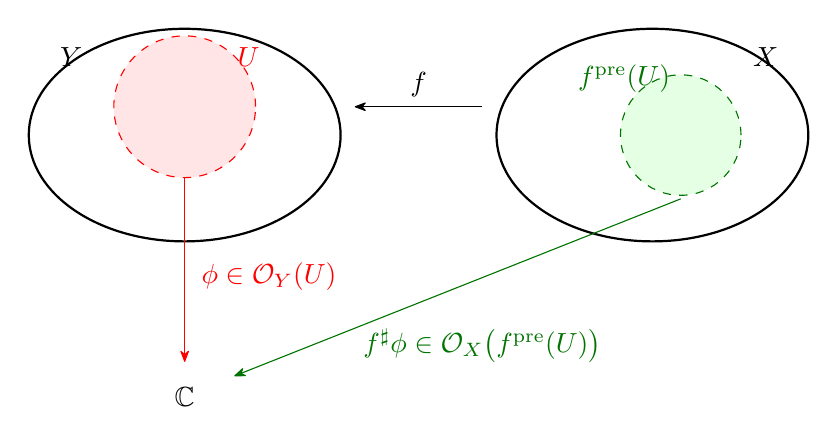
\begin{tikzpicture}[scale=0.9,>={Stealth[round]}]
  % X (right blob) and its open preimage
  \draw[thick] (2.6,0) ellipse (2.2 and 1.5);
  \node at (4.2,1.1) {$X$};
  \draw[green!45!black,dashed,fill=green!20,fill opacity=0.5] (3.0,0) circle (0.85);
  \node[green!45!black] at (2.2,0.8) {$f^{\mathrm{pre}}(U)$};
  % Y (left blob) and its open set U
  \draw[thick] (-4.0,0) ellipse (2.2 and 1.5);
  \node at (-5.6,1.1) {$Y$};
  \draw[red,dashed,fill=red!20,fill opacity=0.5] (-4.0,0.4) circle (1.0);
  \node[red] at (-3.1,1.1) {$U$};
  % f : X -> Y
  \draw[->] (0.2,0.4) -- (-1.6,0.4) node[midway,above] {$f$};
  % phi : U -> C
  \draw[red,->] (-4.0,-0.6) -- (-4.0,-3.2);
  \node[red,right] at (-3.9,-2.0) {$\phi \in \mathcal O_Y(U)$};
  \node at (-4.0,-3.7) {$\mathbb C$};
  % f-sharp phi
  \draw[green!45!black,->] (3.0,-0.9) -- (-3.3,-3.4);
  \node[green!45!black,below] at (0.2,-2.6)
    {$f^\sharp \phi \in \mathcal O_X\bigl(f^{\mathrm{pre}}(U)\bigr)$};
\end{tikzpicture}
\end{document}
